
\subsection{Degree Distribution and Power Law}
% BEGIN: degree distribution and power law

% END: degree distribution and power law

\subsection{Most Important Symptoms/Diseases (4 Classes)}
% BEGIN: most important symptoms/diseases (4 classes)

% END: most important symptoms/diseases (4 classes)

\subsection{Betweenness Centrality}
% BEGIN: betweenness centrality
As shown in Figure \ref{fig:bet_entire}, the betweenness centrality of the nodes in the network follows a Power Law Distribution. This suggests
a scale-free structure of the network, with a few central nodes working as connecting actors, while the majority of the nodes have a low betweenness centrality.
Dividing the centrality values into the two classes of symptoms and diseases (Figures \ref{fig:bet_diseases} and \ref{fig:bet_symptoms}), we can see that 
the symptoms have a higher betweenness centrality than the diseases. To understand the meaning of this result we have to delve into
the interpretation of the betweenness centrality. In general, a symptom is more likely to have a high betweenness centrality if it is
connected to many diseases and these latter are connected to few symptoms. Conversely a disease is more likely to have a high betweenness centrality
if it is connected to many symptoms and these latter are connected to few diseases. Looking at the results of L1 and L2, we can see that in our case
the justification of the higher symptoms betweenness centrality is due to the fact that the symptoms are connected to many diseases, while the diseases
are connected to few symptoms.
From a predictive point of view, this is not a good result, since each symptom is not very specific contributing to many different classes.

Figure \ref{fig:bet_top} shows the top 10 nodes with the highest betweenness centrality. As expected, they are all symptoms and seems 
reasonable that they are the most generic symptoms.

\begin{figure}[H]
    \centering
    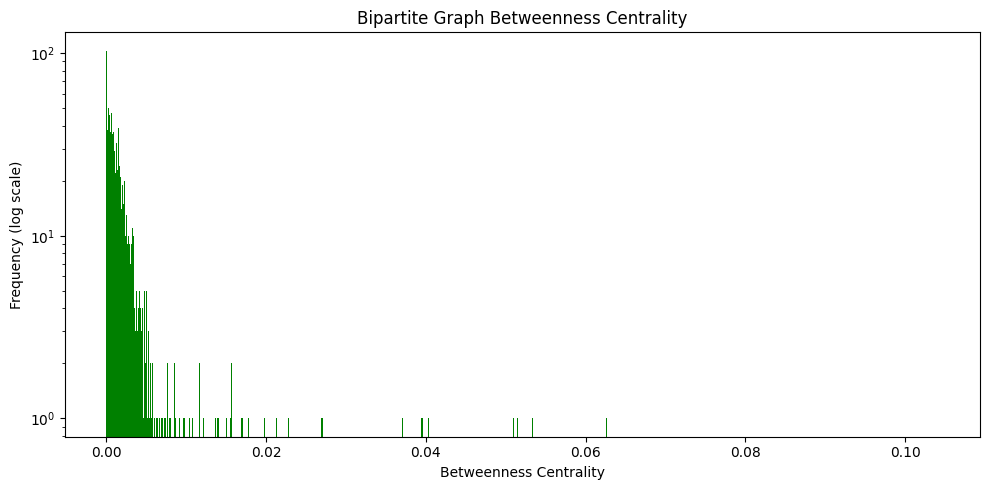
\includegraphics[width=1\columnwidth]{bet_entire.png}
    \caption{Betweenness Centrality of the entire network}
    \label{fig:bet_entire}
\end{figure}

\begin{figure}[H]
    \centering
    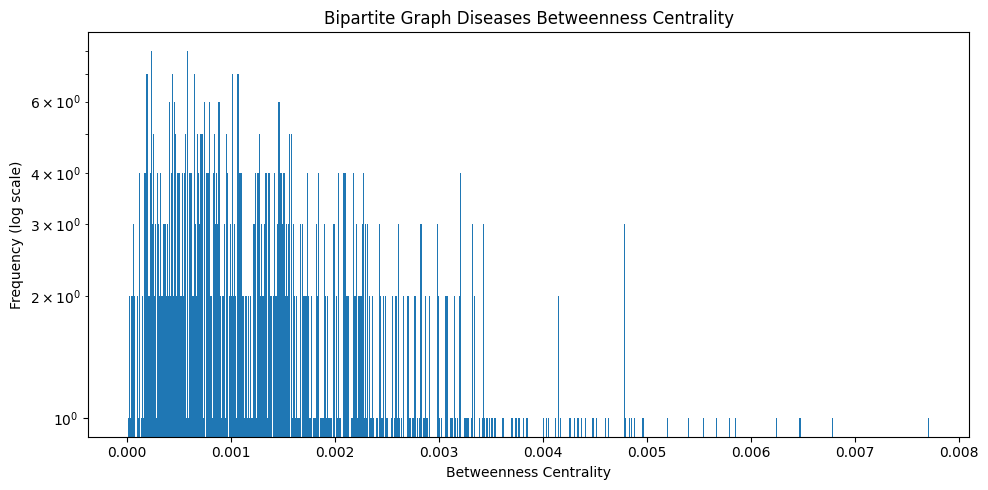
\includegraphics[width=1\columnwidth]{bet_diseases.png}
    \caption{Betweenness Centrality of the diseases}
    \label{fig:bet_diseases}
\end{figure}

\begin{figure}[H]
    \centering
    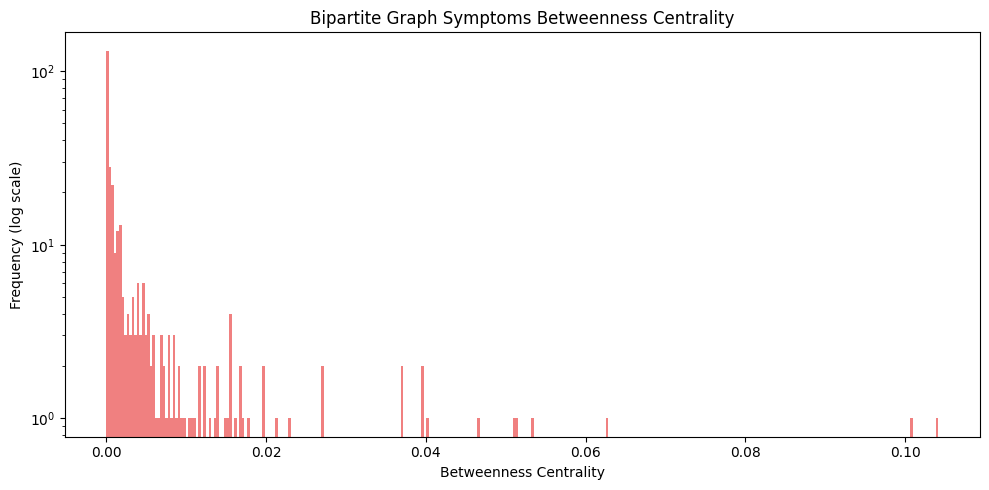
\includegraphics[width=1\columnwidth]{bet_symptoms.png}
    \caption{Betweenness Centrality of the symptoms}
    \label{fig:bet_symptoms}
\end{figure}

\begin{figure}[H]
   \centering
   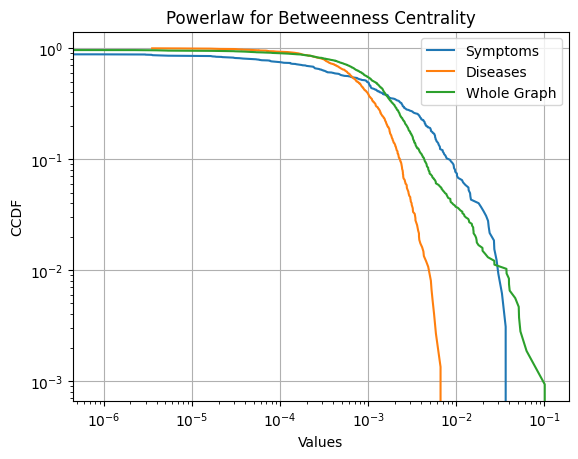
\includegraphics[width=1\columnwidth]{bet_all.png}
   \caption{Betweenness Centrality CDFs}
   \label{fig:bet_all}
\end{figure}

\begin{figure}[H]
    \centering
    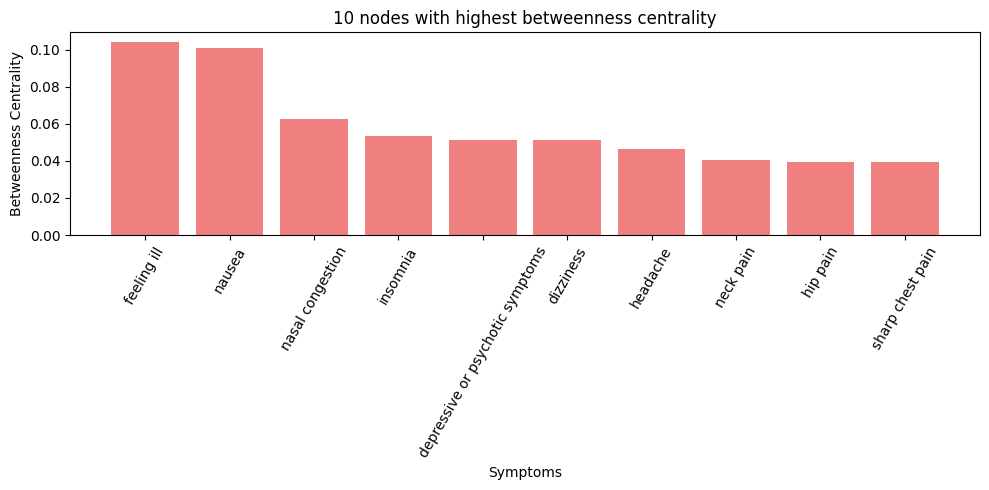
\includegraphics[width=1\columnwidth]{bet_top.png}
    \caption{Top 10 nodes with the highest betweenness centrality}
    \label{fig:bet_top}
\end{figure}

% END: betweenness centrality

\subsection{Communities}
% BEGIN: communities
The detection of communities in a network can be useful both for the interpretation of the network itself and for the ML model prediction Enhancing.
As regard the network interpretation it is worth to underline that a community of symptoms identifies a set of symptoms that are 
often co-occurring within the same diseases, while a community of diseases identifies a set of diseases that are often co-occurring within the same symptoms.
In Figure \ref{fig:com_sizes_all} we can see the sizes comparison of the communities of symptoms and diseases. It is clear that the diseases communities are


Starting from the analysis of the symptoms communities, we can see that the symptoms are grouped in 3 communities (Figures \ref{fig:com1_symptoms}, 
\ref{fig:com2_symptoms} and \ref{fig:com3_symptoms}). Each figure shows the diseases to which most different symptoms point.


\begin{figure}[H]
    \centering
    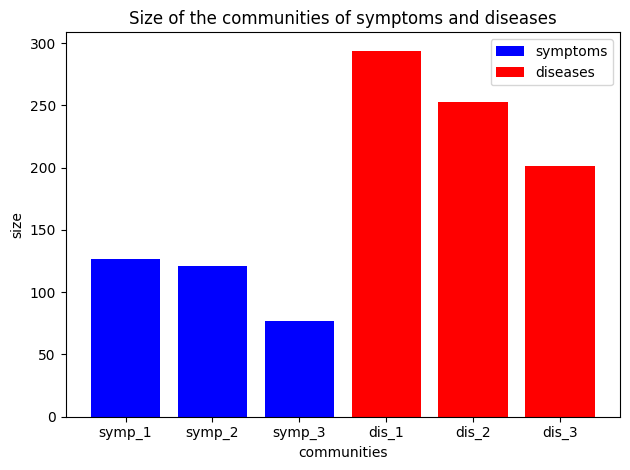
\includegraphics[width=1\columnwidth]{com_sizes_all.png}
    \caption{Sizes of the communities of symptoms and diseases}
    \label{fig:com_sizes_all}
\end{figure}

\begin{figure}[H]
    \centering
    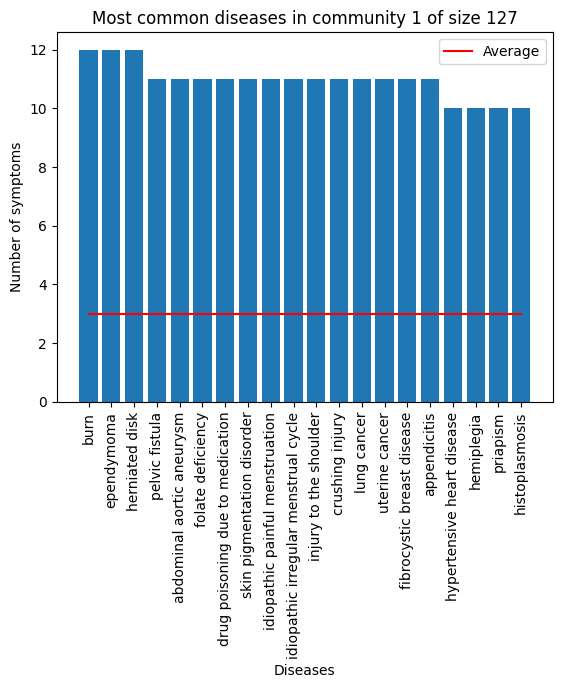
\includegraphics[width=1\columnwidth]{com1_symptoms.png}
    \caption{Community 1 of symptoms}
    \label{fig:com1_symptoms}
\end{figure}

\begin{figure}[H]
    \centering
    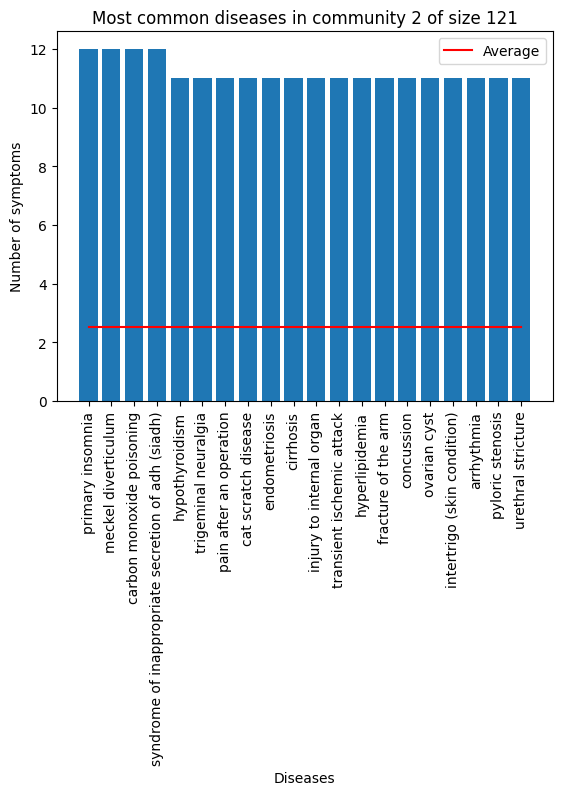
\includegraphics[width=1\columnwidth]{com2_symptoms.png}
    \caption{Community 2 of symptoms}
    \label{fig:com2_symptoms}
\end{figure}

\begin{figure}[H]
    \centering
    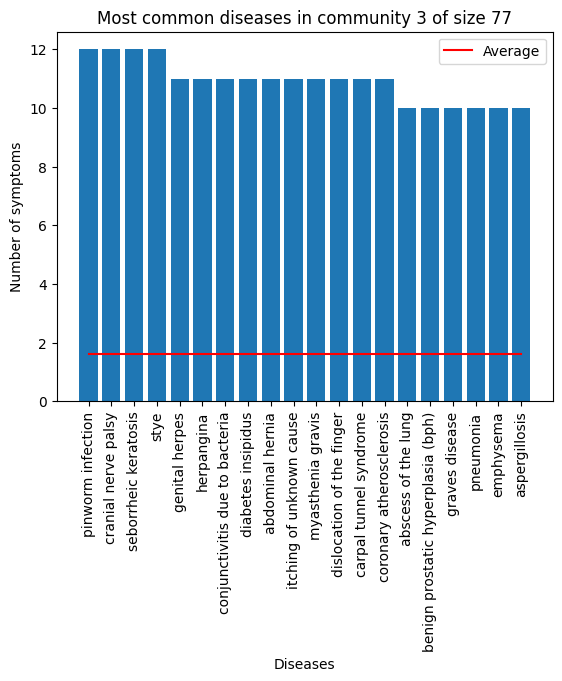
\includegraphics[width=1\columnwidth]{com3_symptoms.png}
    \caption{Community 3 of symptoms}
    \label{fig:com3_symptoms}
\end{figure}


% END: communities


